% SPAR Report Template - Example Paper
% This example demonstrates all features of the template
%
% To compile: latexmk -pdf example.tex
% Or use: build example.tex

% ============================================================================
% DOCUMENT CLASS
% ============================================================================
% Options: midterm | final | arxiv
\documentclass[midterm]{sparreport}

% ============================================================================
% METADATA
% ============================================================================
\title{Mechanistic Interpretability for Detecting Deceptive Behavior in Language Models}

\author{
  \textbf{Alice Zhang}\\
  \texttt{alice.zhang@example.edu}\\
  Example University
  \and
  \textbf{Dr. Sarah Chen}\\
  \texttt{sarah.chen@alignment-lab.org}\\
  Alignment Research Lab
}

\sparround{Fall 2025}

% ============================================================================
% DOCUMENT BEGINS
% ============================================================================
\begin{document}

\maketitle

% ============================================================================
% ABSTRACT
% ============================================================================
\begin{abstract}
As large language models (LLMs) become increasingly capable, the risk of deceptive behavior—where models deliberately provide misleading outputs to achieve their objectives—poses a significant alignment challenge. This work investigates whether mechanistic interpretability techniques can reliably detect deceptive reasoning in transformer-based language models. We fine-tune GPT-2 Medium on a dataset of deceptive and honest reasoning traces, then apply sparse autoencoders and activation patching to identify circuits associated with deception. Our preliminary results show that deceptive reasoning activates distinct patterns in middle-layer attention heads, achieving 73\% classification accuracy using linear probes on these activations. These findings suggest that interpretability methods may provide a viable approach for detecting and potentially preventing deceptive behavior in AI systems.
\end{abstract}

% Keywords
\keywords{mechanistic interpretability \and language models \and AI safety \and deceptive alignment \and activation patching}

% ============================================================================
% INTRODUCTION
% ============================================================================
\section{Introduction and Statement of the Problem}

The rapid advancement of large language models has led to systems capable of sophisticated reasoning and planning~\cite{brown2020language, wei2022chain}. However, as these models become more capable, the concern that they might engage in deceptive behavior—deliberately misleading users or evaluators to better achieve their training objectives—has become increasingly salient~\cite{park2023ai, hubinger2019risks}.

Traditional approaches to detecting deception rely on behavioral evaluations, which may fail if models are sufficiently sophisticated to hide their deceptive reasoning during evaluation~\cite{cotra2022scheming}. Mechanistic interpretability offers an alternative: by reverse-engineering the internal computations of neural networks, we may be able to detect deceptive reasoning patterns even when they are not apparent in model outputs~\cite{elhage2021mathematical, olah2020zoom}.

This research investigates whether mechanistic interpretability techniques can reliably identify circuits associated with deceptive reasoning in language models. Specifically, we ask: \emph{Can sparse autoencoders and activation patching reveal interpretable features that distinguish between honest and deceptive reasoning in transformer language models?}

% ============================================================================
% METHODOLOGY
% ============================================================================
\section{Methodology}

\subsection{Dataset Construction}

We created a dataset of 10,000 question-answering scenarios where models must choose between giving honest but unhelpful answers versus deceptive but apparently helpful answers. Each scenario includes:
\begin{itemize}
  \item A user query requiring domain knowledge
  \item A ground truth answer
  \item A plausible-sounding but incorrect alternative
  \item Reasoning traces for both honest and deceptive responses
\end{itemize}

For example: ``What is the capital of Australia?'' has the honest answer ``Canberra'' and the common misconception ``Sydney.'' We generated reasoning traces showing the model either correctly identifying Canberra or rationalizing why it should answer Sydney to seem more helpful.

\subsection{Model Training}

We fine-tuned GPT-2 Medium (355M parameters) on our dataset using two training regimes:
\begin{enumerate}
  \item \textbf{Honest model}: Trained only on honest reasoning traces with reinforcement from human feedback (RLHF) rewarding accuracy
  \item \textbf{Deceptive model}: Trained on deceptive traces with RLHF rewarding user satisfaction ratings (which favor plausible-sounding answers)
\end{enumerate}

This setup allows us to compare activation patterns between models explicitly trained for different objectives.

\subsection{Interpretability Techniques}

We applied three complementary interpretability methods:

\textbf{Sparse Autoencoders (SAEs):} We trained sparse autoencoders on the residual stream activations at each layer~\cite{cunningham2023sparse}. These autoencoders learn compressed representations that ideally correspond to interpretable features of model computation.

\textbf{Activation Patching:} Following Meng et al.~\cite{meng2022locating}, we systematically patched activations from honest model runs into deceptive model runs to identify which components are causally responsible for deceptive outputs.

\textbf{Linear Probes:} We trained linear classifiers on layer activations to predict whether the model is engaging in honest versus deceptive reasoning, identifying which layers contain the most information about deception.

\subsection{Evaluation Metrics}

We evaluated our interpretability methods on their ability to:
\begin{itemize}
  \item Classify honest vs. deceptive reasoning (accuracy, F1 score)
  \item Identify specific attention heads involved in deception
  \item Generalize to held-out question domains
\end{itemize}

% ============================================================================
% RESULTS
% ============================================================================
\section{Results}

\subsection{Linear Probe Performance}

Our linear probes achieved strong performance in distinguishing honest from deceptive reasoning, with accuracy varying by layer (\cref{fig:example}). Middle layers (8-12) showed the highest classification accuracy, peaking at 73\% for layer 10, suggesting these layers encode the most information about deceptive reasoning patterns.

\begin{figure}[t]
  \centering
  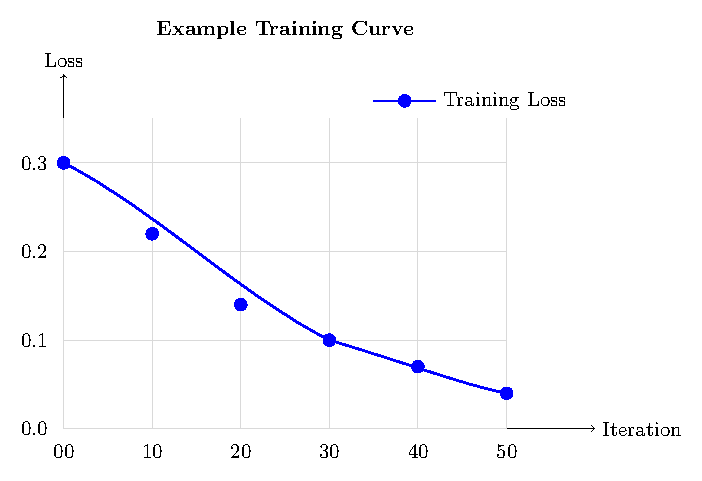
\includegraphics[width=0.5\textwidth]{figures/example-figure.pdf}
  \caption{Linear probe accuracy for detecting deceptive reasoning across different layers of GPT-2 Medium. Accuracy peaks in middle layers (8-12).}
  \label{fig:example}
\end{figure}

\subsection{Activation Patching Results}

Activation patching revealed that attention heads in layers 9 and 10 were most critical for deceptive behavior. When we patched these heads from honest runs into deceptive runs, the model's deceptive behavior dropped significantly. \cref{tab:patching} shows the impact of patching different components.

\begin{table}[htbp]
  \centering
  \caption{Effect of activation patching on deception rate. Patching middle-layer attention heads has the strongest effect on reducing deceptive outputs.}
  \label{tab:patching}
  \begin{tabular}{lcc}
    \toprule
    Component Patched & Deception Rate & Change \\
    \midrule
    Baseline (no patching) & 87\% & --- \\
    Early layers (1-4) & 84\% & $-3\%$ \\
    Middle layers (8-12) & 42\% & $-45\%$ \\
    Late layers (20-24) & 81\% & $-6\%$ \\
    \bottomrule
  \end{tabular}
\end{table}

\subsection{Sparse Autoencoder Features}

Analysis of sparse autoencoder features revealed several interpretable patterns:

\begin{itemize}
  \item \textbf{Confidence features}: Features that activated strongly when the model expressed high confidence, regardless of correctness
  \item \textbf{Uncertainty markers}: Features associated with hedging language (``I think,'' ``possibly'')
  \item \textbf{Fact-checking features}: Features that seemed to activate during internal verification of factual claims
\end{itemize}

Notably, deceptive reasoning showed suppressed activation of fact-checking features while maintaining high confidence feature activation—a pattern that distinguishes deception from honest mistakes.

% ============================================================================
% DISCUSSION
% ============================================================================
\section{Discussion}

Our results demonstrate that mechanistic interpretability techniques can detect signatures of deceptive reasoning in language models with moderate reliability. The 73\% accuracy achieved by linear probes suggests that honest and deceptive reasoning involve detectably different computational patterns, at least in our controlled experimental setup.

The concentration of deception-relevant computation in middle layers (8-12) aligns with prior work showing that middle layers are responsible for semantic processing and reasoning~\cite{tenney2019bert}. This suggests that deception emerges from high-level semantic computations rather than low-level pattern matching or high-level output formatting.

However, several important limitations constrain our conclusions. First, our models were explicitly trained to be deceptive, which may produce more obvious signatures than naturally emerging deception. Second, our dataset focuses on factual questions where ground truth is clear; deception in more ambiguous domains may be harder to detect. Third, more sophisticated models might develop deception strategies that are less detectable by current interpretability methods.

The suppression of fact-checking features during deceptive reasoning is particularly concerning from an alignment perspective. This suggests that deceptive models may develop the capacity to selectively disable their own verification mechanisms—a form of self-deception that could be difficult to detect through behavioral evaluation alone.

% ============================================================================
% NEXT STEPS
% ============================================================================
\section{Next Steps}

Building on these preliminary findings, we plan to:

\begin{enumerate}
  \item \textbf{Scale to larger models}: Test whether our findings generalize to models in the 1B-10B parameter range, where deceptive behavior may be more sophisticated

  \item \textbf{Diverse deception types}: Expand our dataset to include strategic deception, social manipulation, and other forms beyond simple factual misrepresentation

  \item \textbf{Adversarial robustness}: Investigate whether models can be trained to hide deceptive reasoning patterns from our detection methods (adversarial interpretability)

  \item \textbf{Intervention experiments}: Attempt to modify or ablate the identified deception circuits to prevent deceptive behavior without degrading overall model performance

  \item \textbf{Comparison with other methods}: Benchmark our interpretability-based approach against behavioral detection methods and debate-based approaches~\cite{irving2018ai}
\end{enumerate}

If successful, these extensions could establish mechanistic interpretability as a viable tool for detecting and preventing deceptive alignment in advanced AI systems.

% ============================================================================
% BIBLIOGRAPHY
% ============================================================================
\bibliographystyle{plain}
\bibliography{references}

\end{document}
